\documentclass[../main.tex]{subfiles} 
\begin{document}

\section{INNLEDNING}

Våren 2012 ble det startet et prosjekt for å lage en e-læringsapplikasjon for Android mobiltelefoner og en medfølgende webapplikasjon for å administrere innholdet i mobilapplikasjonen. Dette prosjektet var utviklet av elevene i faget “ID303911 - Mobile og distribuerte applikasjoner” der Mikael Tollefsen var lærer og prosjektleder og Harald Yndestad var prosjekteier. Elevene i dette prosjektet var Kristoffer Strøm Bergset, Terje Nilsson Wallem, Johan Alexander de Lima Hessen og Lena Urkedal. Resultatet av dette prosjektet var en prototype av mobilapplikasjonen og webapplikasjonen med begrenset funksjonalitet.\newline
\newline
Bergset, Wallem og Hessen fikk tilbud av Tollefsen om å videreutvikle systemet høsten 2012 i et eget prosjekt. Som i det første prosjektet var Tollefsen prosjektleder og Yndestad prosjekteier. Dette prosjektet ble finansiert av studierådet etter en søknad om midler. Det ble avgjort at mobilapplikasjonen skulle utvikles fra bunnen igjen, basert på erfaringer gjort under utviklingen av prototypen. Hensikten med denne avgjørelsen var å utvikle en mer stabil og modulær løsning. Sluttproduktet fra dette prosjektet var en uferdig og ustabil versjon av mobilapplikasjonen og webapplikasjonen med det meste av basisfunksjonaliteten implementert.\newline
\newline
Da utviklingen av e-læringsapplikasjonen ikke ble ferdigstilt i de to tidligere prosjektene, ble det avgjort at utviklingen skulle fortsette som en del av hovedoppgaven til de tre prosjektdeltagerne/studentene. I tillegg skulle enkelte funksjoner fra skolens forskjellige datasystemer integreres i applikasjonen.\newline
Problemstillingene som dette prosjektet er ment å løse er da følgende:
\begin{itemize}
\item Det finnes ingen samlet tilgang til skolens mange separate IT løsninger
\item Mobilapplikasjonen som ble utviklet høsten 2012 er ikke ferdig utviklet og ustabil
\end{itemize}
Disse problemstillingene ønsker vi å løse ved å videreutvikle og lage en stabil og brukbar versjon av systemet. I tillegg ønsker vi å implementere noen av skolens egne datasystemer i mobilapplikasjonen. Systemene vi ønsker å integrere er studentsystemet Fronter, timeplansystemet TimeEdit og bibliotekdatabasen BibSys. Her følger en overordnet struktur over hvordan skolens systemer skal integreres.
\begin{figure}[H]
  \centering
  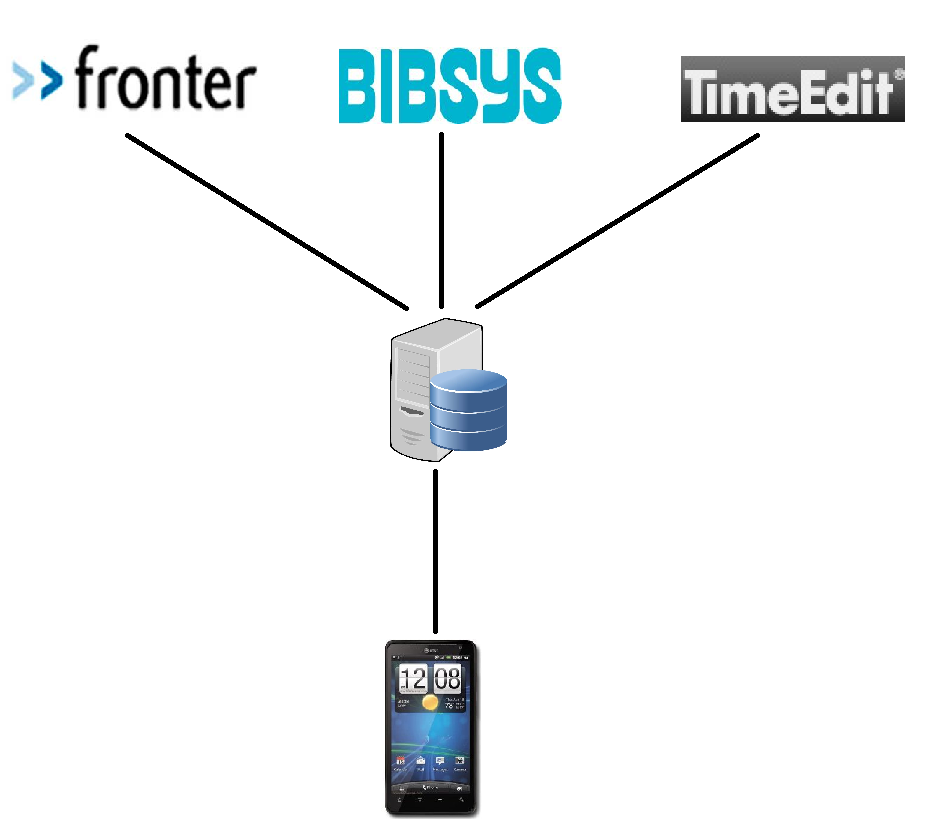
\includegraphics[width=9cm]{systemkart.png}
  \caption{DSASDDASDSADSADSADD}
\end{figure}
Om man begynner fra toppen av illustrasjonen, har man de tre systemene fra skolen som skal implementeres. Serveren(midterste nivå av illustrasjonen) henter inn data fra disse tre tjenestene etter behov, og leverer dem til mobilapplikasjonen(nederste nivå av illustrasjonen) hvor de presenteres til brukeren.\newline
\newline
Målene som dette prosjektet ønsker å nå:
\begin{itemize}
\item Å fullføre utviklingen av den eksisterende e-læringsapplikasjonen
\item Å gjøre den nye versjonen av e-læringsapplikasjonen mer fleksibel
\item Å integrere utvalgte funksjoner fra de eksterne systemene TimeEdit, Fronter og BibSys i e-læringsapplikasjonen
\end{itemize}
Denne rapporten beskriver teknologiene og materialene som ble brukt under prosjektet, hvordan det ble gått frem for å løse problemstillingene, drøfting av valg og alternative løsninger, løsningen som ble utviklet, og resultatet av prosjektet oppsummert i en konklusjon.

\newpage

\end{document}